% Options for packages loaded elsewhere
\PassOptionsToPackage{unicode}{hyperref}
\PassOptionsToPackage{hyphens}{url}
%
\documentclass[
  letterpaper,
  ignorenonframetext,
  aspectratio=43,
  handout,
  12pt]{beamer}
\usepackage{pgfpages}
\setbeamertemplate{caption}[numbered]
\setbeamertemplate{caption label separator}{: }
\setbeamercolor{caption name}{fg=normal text.fg}
\beamertemplatenavigationsymbolsempty
% Prevent slide breaks in the middle of a paragraph
\widowpenalties 1 10000
\raggedbottom
\setbeamertemplate{part page}{
  \centering
  \begin{beamercolorbox}[sep=16pt,center]{part title}
    \usebeamerfont{part title}\insertpart\par
  \end{beamercolorbox}
}
\setbeamertemplate{section page}{
  \centering
  \begin{beamercolorbox}[sep=12pt,center]{part title}
    \usebeamerfont{section title}\insertsection\par
  \end{beamercolorbox}
}
\setbeamertemplate{subsection page}{
  \centering
  \begin{beamercolorbox}[sep=8pt,center]{part title}
    \usebeamerfont{subsection title}\insertsubsection\par
  \end{beamercolorbox}
}
\AtBeginPart{
  \frame{\partpage}
}
\AtBeginSection{
  \ifbibliography
  \else
    \frame{\sectionpage}
  \fi
}
\AtBeginSubsection{
  \frame{\subsectionpage}
}
\usepackage{amsmath,amssymb}
\usepackage{lmodern}
\usepackage{ifxetex,ifluatex}
\ifnum 0\ifxetex 1\fi\ifluatex 1\fi=0 % if pdftex
  \usepackage[T1]{fontenc}
  \usepackage[utf8]{inputenc}
  \usepackage{textcomp} % provide euro and other symbols
\else % if luatex or xetex
  \usepackage{unicode-math}
  \defaultfontfeatures{Scale=MatchLowercase}
  \defaultfontfeatures[\rmfamily]{Ligatures=TeX,Scale=1}
\fi
\usetheme[]{metropolis}
% Use upquote if available, for straight quotes in verbatim environments
\IfFileExists{upquote.sty}{\usepackage{upquote}}{}
\IfFileExists{microtype.sty}{% use microtype if available
  \usepackage[]{microtype}
  \UseMicrotypeSet[protrusion]{basicmath} % disable protrusion for tt fonts
}{}
\makeatletter
\@ifundefined{KOMAClassName}{% if non-KOMA class
  \IfFileExists{parskip.sty}{%
    \usepackage{parskip}
  }{% else
    \setlength{\parindent}{0pt}
    \setlength{\parskip}{6pt plus 2pt minus 1pt}}
}{% if KOMA class
  \KOMAoptions{parskip=half}}
\makeatother
\usepackage{xcolor}
\IfFileExists{xurl.sty}{\usepackage{xurl}}{} % add URL line breaks if available
\IfFileExists{bookmark.sty}{\usepackage{bookmark}}{\usepackage{hyperref}}
\hypersetup{
  hidelinks,
  pdfcreator={LaTeX via pandoc}}
\urlstyle{same} % disable monospaced font for URLs
\newif\ifbibliography
\usepackage{graphicx}
\makeatletter
\def\maxwidth{\ifdim\Gin@nat@width>\linewidth\linewidth\else\Gin@nat@width\fi}
\def\maxheight{\ifdim\Gin@nat@height>\textheight\textheight\else\Gin@nat@height\fi}
\makeatother
% Scale images if necessary, so that they will not overflow the page
% margins by default, and it is still possible to overwrite the defaults
% using explicit options in \includegraphics[width, height, ...]{}
\setkeys{Gin}{width=\maxwidth,height=\maxheight,keepaspectratio}
% Set default figure placement to htbp
\makeatletter
\def\fps@figure{htbp}
\makeatother
% Make links footnotes instead of hotlinks:
\DeclareRobustCommand{\href}[2]{#2\footnote{\url{#1}}}
\setlength{\emergencystretch}{3em} % prevent overfull lines
\providecommand{\tightlist}{%
  \setlength{\itemsep}{0pt}\setlength{\parskip}{0pt}}
\setcounter{secnumdepth}{-\maxdimen} % remove section numbering
\usepackage{pgfpages}
\pgfpagesuselayout{2 on 1}
\providecommand{\tightlist}{%
\setlength{\itemsep}{0pt}\setlength{\parskip}{0pt}}
\makeatletter
\makeatother
\let\Oldincludegraphics\includegraphics
\renewcommand{\includegraphics}[2][]{\Oldincludegraphics[width=\textwidth,height=0.7\textheight,keepaspectratio]{#2}}
\ifluatex
  \usepackage{selnolig}  % disable illegal ligatures
\fi

\author{}
\date{}

\begin{document}

\begin{frame}{Mechanics of Materials}
\protect\hypertarget{mechanics-of-materials}{}
Lecture 9 - Torsion

Dr.~Nicholas Smith

Wichita State University, Department of Aerospace Engineering

3 March, 2021
\end{frame}

\begin{frame}{schedule}
\protect\hypertarget{schedule}{}
\begin{itemize}
\tightlist
\item
  3 Mar - Torsion
\item
  5 Mar - Homework 3 Due
\item
  8 Mar - Torsion
\item
  10 Mar - Bending
\item
  12 Mar - Homework 4 Due, Homework 3 Self-grade due
\end{itemize}
\end{frame}

\begin{frame}{outline}
\protect\hypertarget{outline}{}
\begin{itemize}
\tightlist
\item
  torsion
\item
  power transmission
\item
  group problems
\end{itemize}
\end{frame}

\hypertarget{torsion}{%
\section{torsion}\label{torsion}}

\begin{frame}{torsion}
\protect\hypertarget{torsion-1}{}
\begin{itemize}
\tightlist
\item
  Torque is a moment that tends to twist a member about its axis
\item
  For small deformation problems, we assume that the length and radius
  do not change significantly under torsion
\item
  The primary deformation we are concerned with in torsion is the angle
  of twist, denoted with \(\phi\)
\end{itemize}
\end{frame}

\begin{frame}{shear}
\protect\hypertarget{shear}{}
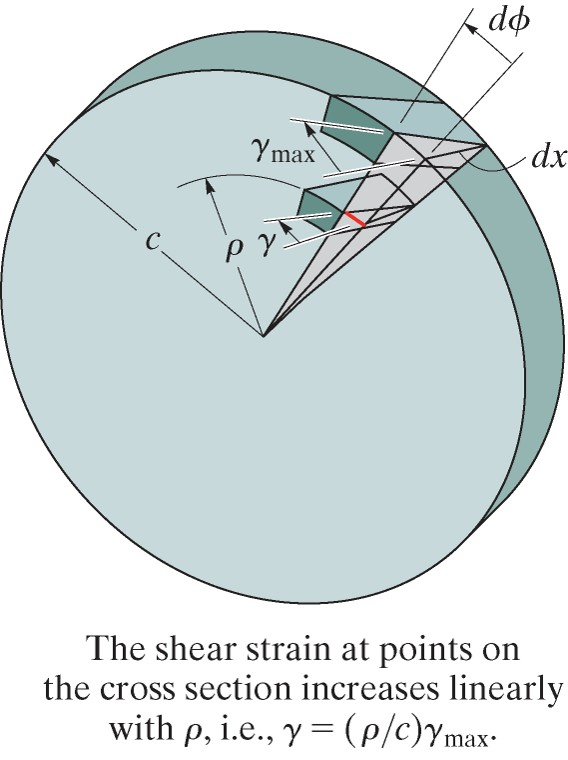
\includegraphics{../images/torsion-disk.jpg}
\end{frame}

\begin{frame}{torsion formula}
\protect\hypertarget{torsion-formula}{}
\begin{itemize}
\tightlist
\item
  For a linearly elastic material, Hooke's Law in shear will hold
  (\(\tau = G \gamma\))
\item
  This means that, like shear strain, shear stress will vary linearly
  along the radius
\end{itemize}
\end{frame}

\begin{frame}{torsion formula}
\protect\hypertarget{torsion-formula-1}{}
\begin{itemize}
\tightlist
\item
  We can find the total force on an element, \emph{dA} by multiplying
  the shear stress by the area
\end{itemize}

\[ dF = \tau dA\]

\begin{itemize}
\tightlist
\item
  The torque (\(dT = \rho dF\)) produced by this force is then
\end{itemize}

\[dT = \rho(\tau dA)\]
\end{frame}

\begin{frame}{torsion formula}
\protect\hypertarget{torsion-formula-2}{}
\begin{itemize}
\tightlist
\item
  Integrating over the whole cross-section gives
\end{itemize}

\[T = \int_A \rho (\tau dA) = \frac{\tau_{max}}{c} \int_A \rho^2 dA\]

\begin{itemize}
\tightlist
\item
  The integral \(\int_A \rho^2 dA\) is also called the Polar Moment of
  Inertia, \emph{J}, so we can write
\end{itemize}

\[\tau_{max} = \frac{Tc}{J}\]
\end{frame}

\begin{frame}{polar moment of inertia}
\protect\hypertarget{polar-moment-of-inertia}{}
\begin{itemize}
\tightlist
\item
  We know that \(J=\int_A \rho^2 dA\), so we can compute this for some
  common shapes
\item
  For a solid circular cross-section, we have
\end{itemize}

\[J = \int_0^c \rho^2 (2\pi \rho d\rho) = \frac{\pi}{2}c^4\]

\begin{itemize}
\tightlist
\item
  For a circular tube we have
\end{itemize}

\[J = \int_{c_1}^{c_2} \rho^2 (2\pi \rho d\rho) = \frac{\pi}{2}(c_2^4-c_1^4)\]
\end{frame}

\begin{frame}{example 5.1}
\protect\hypertarget{example-5.1}{}
\begin{columns}[T]
\begin{column}{0.5\textwidth}
\begin{figure}
\centering
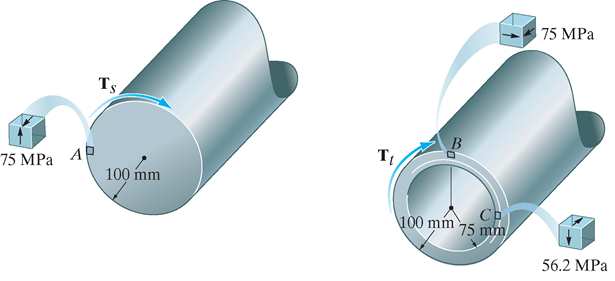
\includegraphics{../images/example-5-1.png}
\caption{On left is a solid 100 mm radius tube, while on the right is a
hollow tube with outer radius of 100 mm and inner radius of 75 mm.
Element A is on the surface of the solid tube on the left, element B is
on the outer surface of the hollow tube on the right and Element C is on
the inner surface of the hollow tube on the right.}
\end{figure}
\end{column}

\begin{column}{0.5\textwidth}
The allowable shear stress is 75 MPa. Determine the maximum torque that
can be applied to each of the cross-sections shown and find the stress
acting on a small element at A, B and C.
\end{column}
\end{columns}
\end{frame}

\hypertarget{power-transmission}{%
\section{power transmission}\label{power-transmission}}

\begin{frame}{power transmission}
\protect\hypertarget{power-transmission-1}{}
\begin{itemize}
\tightlist
\item
  Shafts and tubes are often connected to belts and drives, and the
  torque, speed, and power are all related
\item
  Power is the rate of work done, for rotation problems, \$P = T
  \omega\$
\item
  We are often given the frequency \emph{f} instead of the angular
  velocity, \(\omega\), in this case \$P = 2\pi f T\$
\end{itemize}
\end{frame}

\begin{frame}{power units}
\protect\hypertarget{power-units}{}
\begin{itemize}
\tightlist
\item
  In SI Units, power is expressed in Watts 1 W = 1 N m / sec
\item
  In Freedom Units, power is expressed in Horsepower 1 hp = 550 ft lb /
  sec
\end{itemize}
\end{frame}

\begin{frame}{shaft design}
\protect\hypertarget{shaft-design}{}
\begin{itemize}
\tightlist
\item
  We often know the power and frequency of a drive, and need to design a
  shaft such that the shear stress is acceptable
\item
  We can easily find the torque as \(T=P/2\pi f\), we can use this
  combined with the torsion equation
\end{itemize}

\[\tau_{max} = \frac{Tc}{J}\]

to find the appropriate shaft diameter. - For solid shafts we can solve
for \emph{c} uniquely, but not for hollow shafts
\end{frame}

\begin{frame}{example 5.4}
\protect\hypertarget{example-5.4}{}
\begin{columns}[T]
\begin{column}{0.5\textwidth}
\begin{figure}
\centering
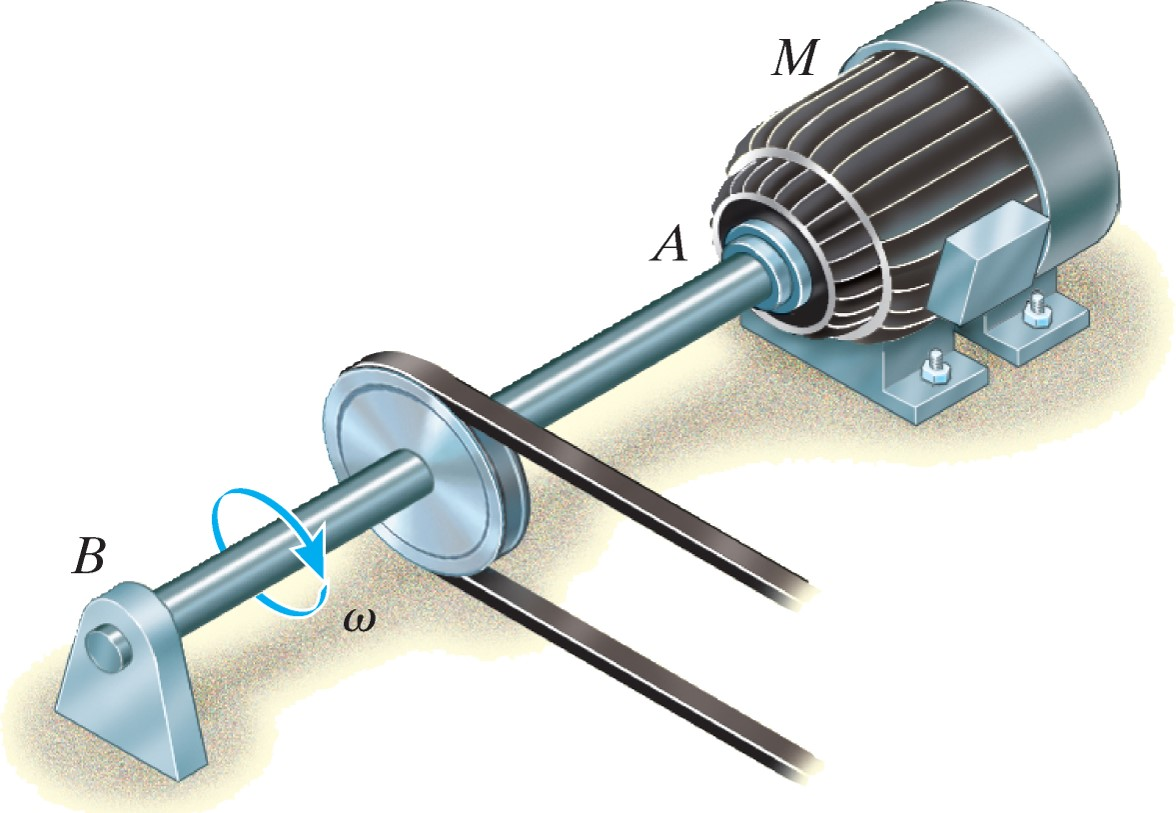
\includegraphics{../images/example-5-4.jpg}
\caption{A rotating shaft connected to a motor}
\end{figure}
\end{column}

\begin{column}{0.5\textwidth}
The steel shaft shown is connected to a 5 hp motor that rotates at
\(\omega=175\) rpm. If \(\tau_{allow}=14.5\) ksi, determine the required
shaft diameter.
\end{column}
\end{columns}
\end{frame}

\hypertarget{group-problems}{%
\section{group problems}\label{group-problems}}

\begin{frame}{group one}
\protect\hypertarget{group-one}{}
\begin{columns}[T]
\begin{column}{0.5\textwidth}
\begin{figure}
\centering
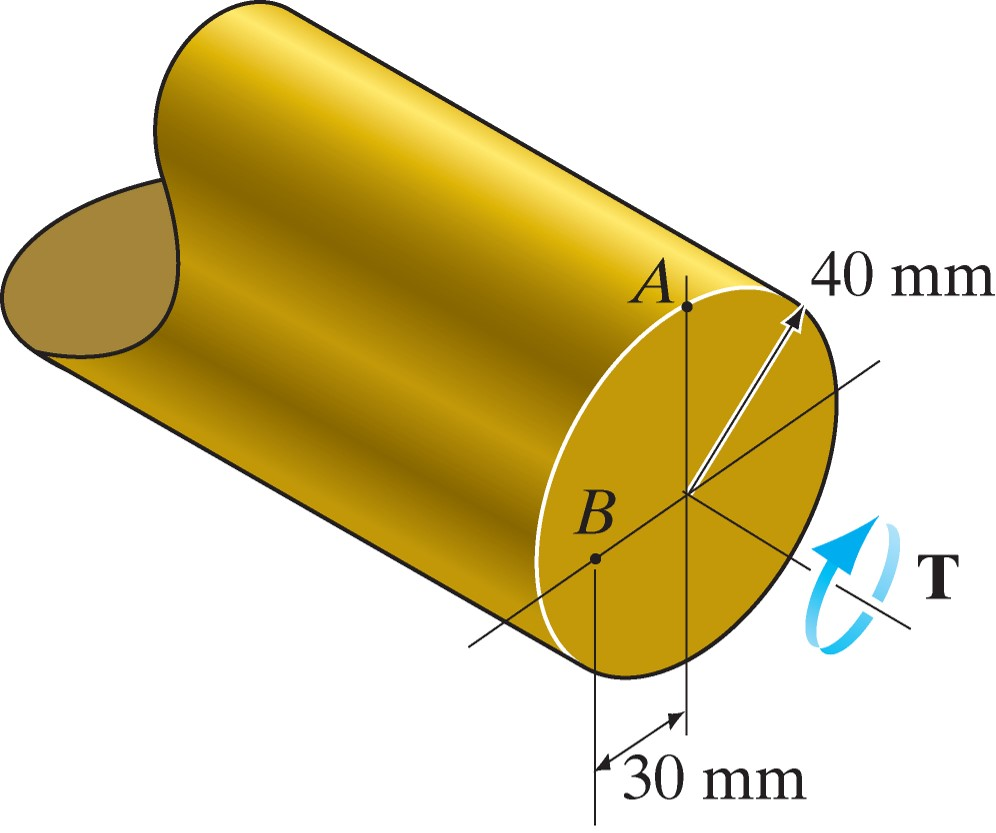
\includegraphics{../images/group5-1.jpg}
\caption{A 40 mm radius solid shaft. Point A is on the outer surface,
Point B is 30 mm away from the center.}
\end{figure}
\end{column}

\begin{column}{0.5\textwidth}
The solid circular shaft is subjected to an internal torque of 5 kN.m.
Determine the shear stress at A and B and represent each state of stress
on a volume element.
\end{column}
\end{columns}
\end{frame}

\begin{frame}{group two}
\protect\hypertarget{group-two}{}
\begin{columns}[T]
\begin{column}{0.5\textwidth}
\begin{figure}
\centering
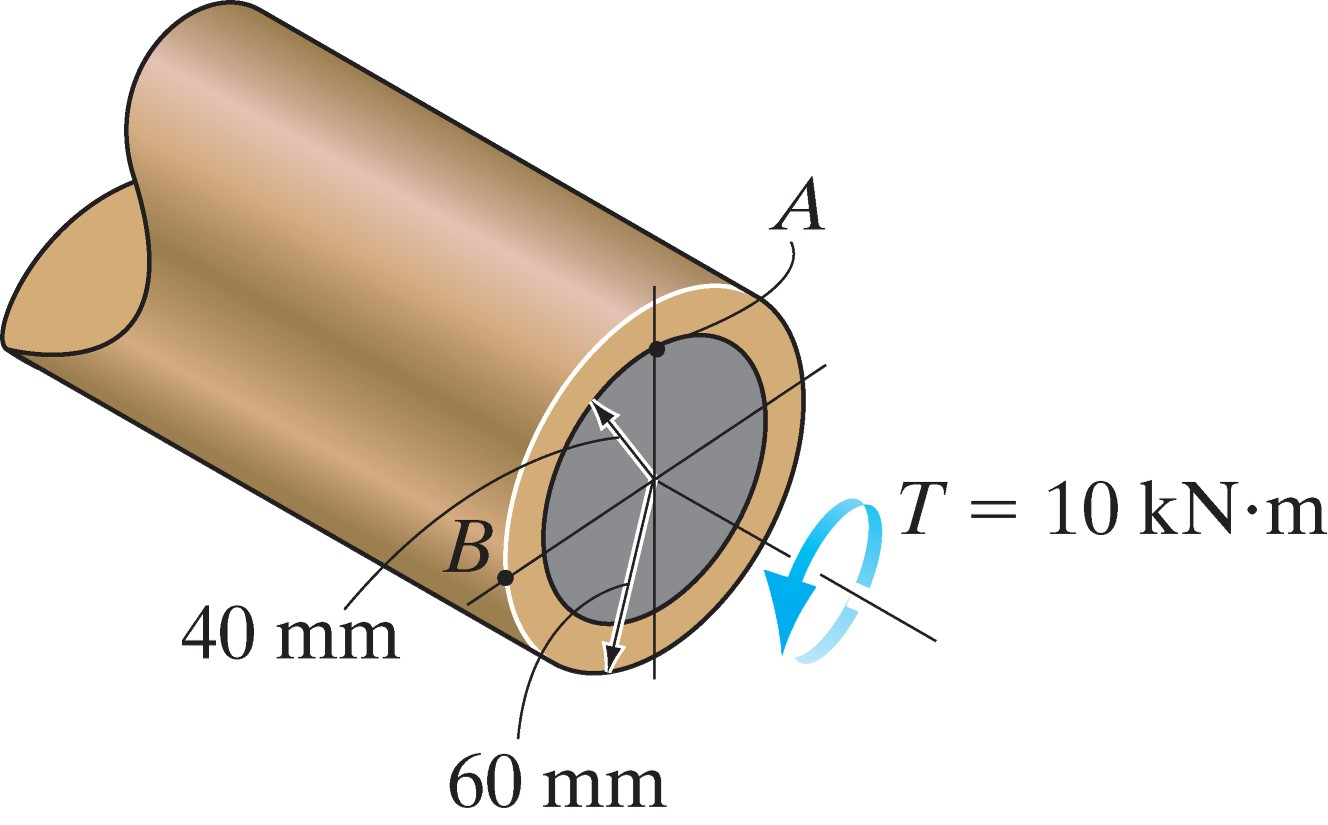
\includegraphics{../images/group5-2.jpg}
\caption{A hollow circular shaft with outer radius of 60 mm and inner
radius of 40 mm. Point A is on the inner surface, Point B is on the
outer surface.}
\end{figure}
\end{column}

\begin{column}{0.5\textwidth}
The hollow circular shaft is subjected to an internal torque of 10 kN.m.
Determine the shear stress at A and B and represent each state of stress
on a volume element.
\end{column}
\end{columns}
\end{frame}

\begin{frame}{group three}
\protect\hypertarget{group-three}{}
\begin{columns}[T]
\begin{column}{0.5\textwidth}
\begin{figure}
\centering
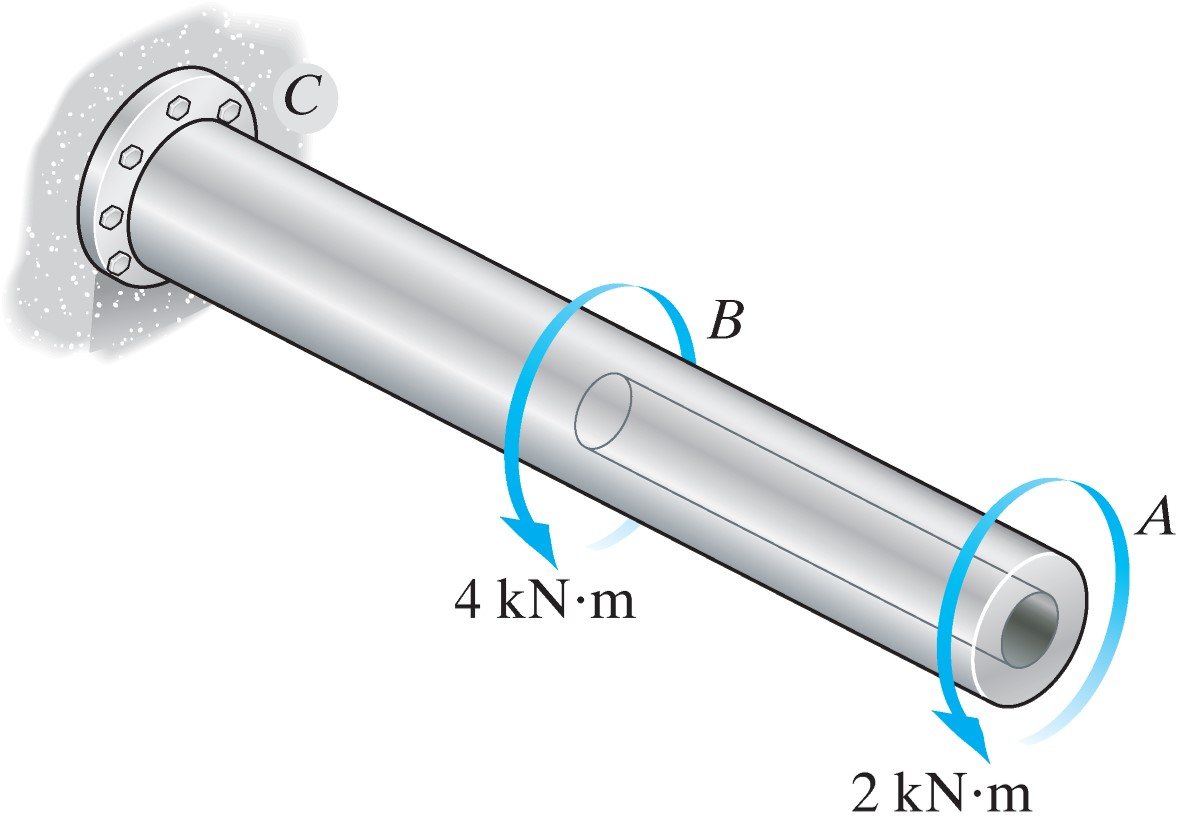
\includegraphics{../images/group5-3.jpg}
\caption{There is a fixed support at C, an applied torque of 4 kN.m at B
(in the middle) and an applied torque of 2 kN.m at A (at the free end).}
\end{figure}
\end{column}

\begin{column}{0.5\textwidth}
The circular shaft is hollow from A to B and solid from B to C.
Determine the shear stress at A and B. The outer diameter is 80 mm and
the wall thickness is 10 mm.
\end{column}
\end{columns}
\end{frame}

\begin{frame}{group four}
\protect\hypertarget{group-four}{}
\begin{columns}[T]
\begin{column}{0.5\textwidth}
\begin{figure}
\centering
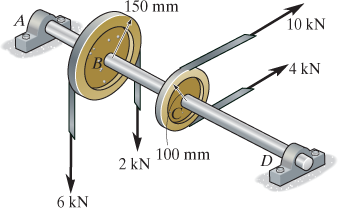
\includegraphics{../images/group-5-4.png}
\caption{A shaft supports to pulleys, one with a 150 mm radius and
tension of 6 kN at one end and 2 kN at the other other. The other pulley
has a 100 mm radius and tensions of 10 kN and 4 kN.}
\end{figure}
\end{column}

\begin{column}{0.5\textwidth}
Determine the maximum shear stress in the 40 mm diameter shaft.
\end{column}
\end{columns}
\end{frame}

\end{document}
